\newpage
\section{TẬP HỢP}
\subsection{LÝ THUYẾT CẦN NHỚ}
\subsubsection{Nhắc lại về tập hợp}
\begin{khung4}{}
	\begin{itemize}
		\item Như đã biết ở cấp Trung học cơ sở, trong toán học, người ta dùng từ \textbf{tập hợp} để chỉ một nhóm đối tượng nào đó hoàn toàn xác định. Mỗi đối tượng trong nhóm gọi là một \textbf{phần tử} của tập hợp đó.
		\item Người ta thường kí hiệu tập hợp bằng các chữ cái in hoa $A$, $B$, $C$, $\ldots$ và kí hiệu phần tử của tập hợp bằng các chữ cái in thường $a$, $b$, $c$, $\ldots$
	\end{itemize}
	\end{khung4}
	\begin{note}
		Đôi khi, để ngắn gọn người ta dùng từ \lq\lq tập\rq\rq\ thay cho \lq\lq tập hợp\rq\rq.
	\end{note}
	\begin{khung4}{}
		\begin{itemize}
			\item Để chỉ $a$ là một phần tử của tập hợp $A$, ta viết $a \in A$ (đọc là \lq\lq$a$ \textbf{thuộc} $A$\rq\rq). Để chỉ $a$ không là phần tử của tập hợp $A$, ta viết $a \notin A$ (đọc là \lq\lq$a$ \textbf{không thuộc} $A$\rq\rq).
			\item Một tập hợp có thể không chứa phần tử nào. Tập hợp như vậy gọi là \textbf{tập rỗng}, kí hiệu $\varnothing$.
			\item Người ta thường kí hiệu các tập hợp số như sau: $\mathbb{N}$ là tập hợp các số tự nhiên; $\mathbb{Z}$ là tập hợp các số nguyên; $\mathbb{Q}$ là tập hợp các số hữu tỉ; $\mathbb{R}$ là tập hợp các số thực.
		\end{itemize}
		\end{khung4}
\indam{Cách xác định tập hợp}
		\begin{khung4}{}
				Xét tập hợp $A$ các số tự nhiên chẵn nhỏ hơn $15$. Ta có thể viết tập hợp $A$ dưới dạng \textbf{liệt kê các phần tử}: \[A=\{0 ; 2 ; 4 ; 6 ; 8 ; 10 ; 12 ; 14\}\]
			hoặc dưới dạng \textbf{chỉ ra tính chất đặc trưng} cho các phần tử
			\[A=\{x \mid x \in \mathbb{N}, x \text { chẵn và } x<15\}.\]
		\end{khung4}
		\begin{note}%[Tex hóa SGK CD-CT,T7/22, Đỗ Minh Phúc]
			Khi liệt kê các phần tử của tập hợp, ta có một số chú ý sau đây
			\begin{enumerate}
				\item Các phần tử có thể được viết theo thứ tự tuỳ ý. Chẳng hạn, để viết tập hợp $A$ các nghiệm của phương trình $x(x-1)=0$, ta có thể viết $A=\{0 ; 1\}$ hoặc $A=\{1 ; 0\}$.
				\item Mỗi phần tử chỉ được liệt kê một lần. Chẳng hạn, nếu kí hiệu $B$ là tập hợp các chữ cái tiếng Anh trong từ \lq\lq \emph{mathematics}\rq\rq\, thì $B=\{m ; a ; t ; h ; e ; i ; c ; s\}$.
				\item Nếu quy tắc xác định các phần tử đủ rõ thì người ta dùng \lq\lq$\ldots$\rq\rq\, mà không nhất thiết viết ra tất cả các phần tử của tập hợp. Chẳng hạn, tập hợp các số tự nhiên không quá $100$ có thể được viết là $\{0 ; 1 ; 2 ; \ldots ; 100\}$.
			\end{enumerate}
		\end{note}
		\begin{luuy}
			Có những tập hợp ta có thể đếm hết các phần tử của chúng. Những tập hợp như vậy được gọi là tập hợp hữu hạn.
			Nếu $E$ là tập hợp hữu hạn thì số phần tử của nó được kí hiệu là $n(E)$. 
			Đặc biệt, $n(\varnothing)=0$.
		\end{luuy}
		\subsubsection{Tập con và hai tập hợp bằng nhau}
		\iconMT\indam{Định nghĩa:}
		\begin{boxdn}
			Cho hai tập hợp $A$ và $B$. Nếu mọi phần tử của $A$ đều là phần tử của $B$ thì ta nói tập hợp $A$ là tập con của tập hợp $B$ và kí hiệu $A \subset B$ (đọc là $A$ chứa trong $B$ ), hoặc $B \supset A$ (đọc là $B$ chứa $A$).
			\end{boxdn}
		\begin{nx}
			\begin{itemize}
				\item $A \subset A$ và $\varnothing \subset A$ với mọi tập hợp $A$.
				\item Nếu $A$ không phải là tập con của $B$ thì ta kí hiệu $A \not \subset B$ (đọc là $A$ không chứa trong $B$ hoặc $B$ không chứa A).
				\item Nếu $A \subset B$ hoặc $B \subset A$ thì ta nói $A$ và $B$ có quan hệ bao hàm.
			\end{itemize}
		\end{nx}
		\begin{khung4}{}
				\immini{Trong toán học, người ta thường minh hoạ tập hợp bằng một hình phẳng được bao quanh bởi một đường cong kín, gọi là biểu đồ Ven (đặt theo tên nhà toán học, nhà triết học người Anh John Venn). Theo cách này, ta có thể minh hoạ $A$ là tập con của $B$ như Hình 1.}{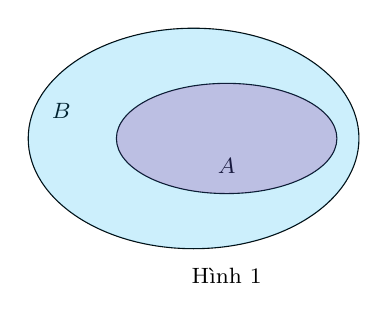
\begin{tikzpicture}[>=stealth,line join=round,line cap=round,font=\footnotesize,scale=.7]
					\coordinate[label=center:$$] (I)at(.4,1);
					\coordinate[label=center:$$] (M)at(1,1);
					\draw (.4,1) circle (3 and 2);
					\coordinate[label=center:$B$] (X)at(-2,1.5);
					\draw (1,1) circle (2 and 1);
					\coordinate[label=center:$A$] (X)at(1,.5);
					\coordinate[label=center:Hình 1] (X)at(1,-1.5);
					\fill[cyan,opacity=.2] (I) ellipse (3 cm and 2 cm)--cycle;
					\fill[violet,opacity=.2] (M) ellipse (2 cm and 1 cm)--cycle;
			\end{tikzpicture}}
		\end{khung4}
		\begin{note}
			\immini {Giữa các tập hợp số quen thuộc (tập số tự nhiên, tập số nguyên, tập số hữu tỉ, tập số thực), ta có quan hệ bao hàm:
				$$\mathbb{N} \subset \mathbb{Z} \subset \mathbb{Q} \subset \mathbb{R}.$$}
			{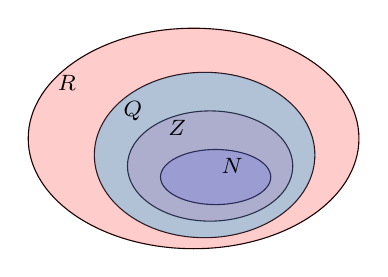
\begin{tikzpicture}[>=stealth,line join=round,line cap=round,font=\footnotesize,scale=.7]
					\path (1.3,1)coordinate[label=center:$$](M) (1.5,.7)coordinate[label=center:$$](N) (1.6,.5)coordinate[label=center:$$](P) (1.7,.3)coordinate[label=center:$$](Q);
					%(1.5,-1.5)coordinate[label=center](H);
					\draw (1.3,1) circle (3 and 2);
					\draw (1.5,.7) circle (2 and 1.5);
					\draw (1.6,.5) circle (1.5 and 1);
					\draw (1.7,.3) circle (1 and .5);
					\fill[red,opacity=.2] (M) ellipse (3 cm and 2 cm)--cycle;
					\fill[cyan,opacity=.3] (N) ellipse (2 cm and 1.5 cm)--cycle;
					\fill[violet,opacity=.1] (P) ellipse (1.5 cm and 1 cm)--cycle;
					\fill[blue,opacity=.1] (Q) ellipse (1 cm and .5 cm)--cycle;
					\coordinate[label=center:$\mathbb{R}$] (X)at(-1,2);
					\coordinate[label=center:$\mathbb{Q}$] (Q)at(0.2,1.5);
					\coordinate[label=center:$\mathbb{Z}$] (Z)at(1,1.2);
					\coordinate[label=center:$\mathbb{N}$] (N)at(2,.5);
			\end{tikzpicture}}
		\end{note}
		\indam{Định nghĩa:}
		\begin{boxdn}
			Hai tập hợp $A$ và $B$ gọi là bằng nhau, kí hiệu $A=B$, nếu $A \subset B$ và $B \subset A$.
		\end{boxdn}
		\begin{luuy}
			Nói cách khác, hai tập hợp $A$ và $B$ bằng nhau nếu mỗi phần tử của tập hợp này cũng là phần tử của tập hợp kia và ngược lại.
		\end{luuy}
			\subsubsection{Một số tập con của tập hợp số thực}
					Cho $a$ và $b$ là hai số thực với $a<b$.
				\begin{center}
					\begin{tabular}{|m{5cm}|m{5cm}|m{7cm}|}
						\hline
						Tên gọi và kí hiệu& Tập hợp& Biểu diễn trên trục số (Phần không bị gạch chéo)
						\\\hline
						Tập số thực $(-\infty;+\infty)$&$\mathbb{R}$&\begin{tikzpicture}[scale=1, font=\footnotesize, line join=round, line cap=round, >=stealth,baseline]
							\draw[->](-1,0)->(5,0);
							\path 
							(2,-0.1)coordinate[label=below:$0$](a) 
							(2,0)coordinate[label=center:$|$](();
						\end{tikzpicture}
						\\\hline
						Đoạn $[a;b]$&$\left\lbrace x \in \mathbb{R} \ \middle|\ a\leq x \leq b\right\rbrace $&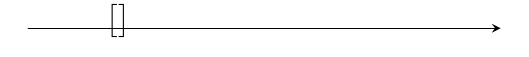
\begin{tikzpicture}[scale=1, font=\footnotesize, line join=round, line cap=round, >=stealth,baseline]
							\draw[->](-1,0)->(5,0);
							\IntervalLR{-1}{1/2}
							\def\skipInterval{0.5cm}
							\IntervalGRF{}{}{\big[}{a}
							\IntervalLR{4}{4.8}
							\def\skipInterval{0.5cm}
							\IntervalGRF{\big]}{b}{}{}
						\end{tikzpicture}
						\\\hline
						Khoảng $(a;b)$&$\left\{x\in\mathbb{R}\ \middle|\ a<x<b\right\}$
						&
						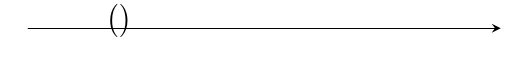
\begin{tikzpicture}[scale=1, font=\footnotesize, line join=round, line cap=round, >=stealth,baseline]
							\draw[->](-1,0)->(5,0);
							\IntervalLR{-1}{1/2}
							\def\skipInterval{0.5cm}
							\IntervalGRF{}{}{\big(}{a}
							\IntervalLR{4}{4.8}
							\def\skipInterval{0.5cm}
							\IntervalGRF{\big)}{b}{}{}
						\end{tikzpicture}
						\\\hline
						Nửa khoảng $[a;b)$&$\left\{x\in\mathbb{R}\ \middle|\ a\leq x<b\right\}$
						&
						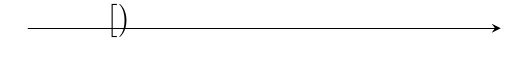
\begin{tikzpicture}[scale=1, font=\footnotesize, line join=round, line cap=round, >=stealth,baseline]
							\draw[->](-1,0)->(5,0);
							\IntervalLR{-1}{1/2}
							\def\skipInterval{0.5cm}
							\IntervalGRF{}{}{\big[}{a}
							\IntervalLR{4}{4.8}
							\def\skipInterval{0.5cm}
							\IntervalGRF{\big)}{b}{}{}
						\end{tikzpicture}
						\\\hline
						Nửa khoảng $(a;b]$&$\left\{x\in\mathbb{R}\ \middle|\ a<x\leq b\right\}$
						&
						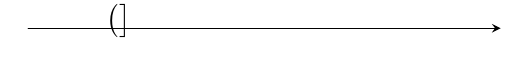
\begin{tikzpicture}[scale=1, font=\footnotesize, line join=round, line cap=round, >=stealth,baseline]
							\draw[->](-1,0)->(5,0);
							\IntervalLR{-1}{1/2}
							\def\skipInterval{0.5cm}
							\IntervalGRF{}{}{\big(}{a}
							\IntervalLR{4}{4.8}
							\def\skipInterval{0.5cm}
							\IntervalGRF{\big]}{b}{}{}
						\end{tikzpicture}
						\\\hline
						Nửa khoảng $(-\infty;a]$&$\left\{x\in\mathbb{R}\ \middle|\ x\leq a\right\}$ &
						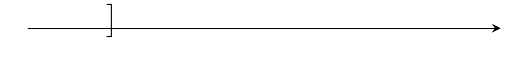
\begin{tikzpicture}[scale=1, font=\footnotesize, line join=round, line cap=round, >=stealth,baseline]
							\draw[->](-1,0)->(5,0);
							\IntervalLR{-1}{1/2}
							\IntervalLR{4}{4.8}
							\def\skipInterval{0.5cm}
							\IntervalGRF{\big]}{a}{}{}
						\end{tikzpicture}
						\\\hline
					\end{tabular}
				\end{center}
				\begin{center}
						\begin{tabular}{|m{5cm}|m{5cm}|m{7cm}|}
						\hline
						Tên gọi và kí hiệu& Tập hợp& Biểu diễn trên trục số (Phần không bị gạch chéo)
						\\\hline
							Nửa khoảng $[a;+\infty)$&$\left\{x\in\mathbb{R}\ \middle|\ x\geq a\right\}$
						&
						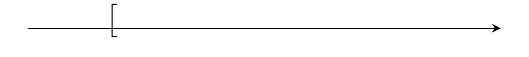
\begin{tikzpicture}[scale=1, font=\footnotesize, line join=round, line cap=round, >=stealth,baseline]
							\draw[->](-1,0)->(5,0);
							\IntervalLR{-1}{1/2}
							\def\skipInterval{0.5cm}
							\IntervalGRF{}{}{\big[}{a}
							\IntervalLR{4}{4.8}
						\end{tikzpicture}
						\\\hline
						Khoảng $(-\infty;a)$&$\left\{x\in\mathbb{R}\ \middle|\ x<a\right\}$ &
						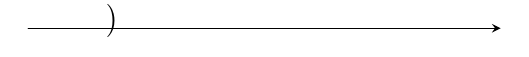
\begin{tikzpicture}[scale=1, font=\footnotesize, line join=round, line cap=round, >=stealth,baseline]
							\draw[->](-1,0)->(5,0);
							\IntervalLR{-1}{1/2}
							\IntervalLR{4}{4.8}
							\def\skipInterval{0.5cm}
							\IntervalGRF{\big)}{a}{}{}
						\end{tikzpicture}
						\\\hline
						Khoảng $(a;+\infty)$&$\left\{x\in\mathbb{R}\ \middle|\ x>a\right\}$
						&
						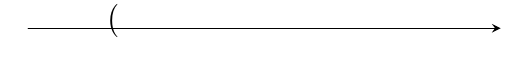
\begin{tikzpicture}[scale=1, font=\footnotesize, line join=round, line cap=round, >=stealth,baseline]
							\draw[->](-1,0)->(5,0);
							\IntervalLR{-1}{1/2}
							\def\skipInterval{0.5cm}
							\IntervalGRF{}{}{\big(}{a}
							\IntervalLR{4}{4.8}
						\end{tikzpicture}
						\\\hline
						\end{tabular}
				\end{center}
				Kí hiệu $-\infty$ đọc là \textbf{âm vô cực}, kí hiệu $+\infty$ đọc là \textbf{dương vô cực}.
	
\subsection{PHÂN LOẠI VÀ PHƯƠNG PHÁP GIẢI TOÁN}
\begin{dang}{Xác định tập hợp}
	\begin{itemize}
  \item Kiểm tra các phần tử thuộc hay không thuộc tập hợp.
  \item Liệt kê các phần tử của tập hợp.
  \item Nêu tính chất đặc trưng của tập hợp.
\end{itemize}
\end{dang}
\begin{vd}%[0D1H2-1]%[Dự án dề cương 3 Khối NH24-25-Đợt 2-Võ Thị Thùy Trang]
	Viết các tập hợp sau đây dưới dang liệt kê các phần tử và tìm số phần tử của mỗi tập hợp đó:
	\begin{enumerate}
		\item Tập hợp $A$ các ước của $24$;
		\item Tập hợp $B$ gồm các chữ số trong số $1\,113\,305$;
		\item $C=\{n \in \mathbb{N} \mid n~ \text{là bội của}~ 5 \text{và}~ n \leq 30\}$;
		\item $D=\left\{x \in \mathbb{R} \mid x^2-2x+3=0\right\}$.
	\end{enumerate}
	\loigiai{
		\begin{enumerate}
		\item $A=\{-24;-12;-8;-6;-4;-3;-2;-1;1;2;3;4;6;8;12;24\}$, $n(A)=16$.
		\item $B=\{0;1;3;5\}$, $n(B)=4$.
		\item $C=\{0;5;10;15;20;25;30\}$, $n(C)=7$.
		\item $D=\varnothing$, $n(D)=0$. Do phương trình $x^2-2x+3=0$ vô nghiệm.	 
		\end{enumerate}
	}
\end{vd}	
\begin{vd}%[0D1H2-1]%[Dự án dề cương 3 Khối NH24-25-Đợt 2-Võ Thị Thùy Trang]
	Viết các tập hợp sau đây dưới dạng chỉ ra tính chất đặc trưng cho các phần tử:
	\begin{enumerate}
		\item $A=\{1; 3; 5; \ldots; 15\}$;
		\item $B=\{0; 5; 10; 15; 20; \ldots\}$;
		\item Tập hợp $C$ các nghiệm của bất phương trình $2x+5> 0$.
	\end{enumerate}
	\loigiai{
		\begin{enumerate}
			\item $A=\{x\mid x~ \text{là số tự nhiên lẻ},\, x\geq 15\}$.
			\item $B=\{n \in \mathbb{N} \mid n~ \text{là bội của } 5\}$.
			\item $C=\{x\in \mathbb{R}\mid 2x+5>0\}$.
		\end{enumerate}
	}
\end{vd}	
\begin{dang}{Tập con và hai tập hợp bằng nhau}	
	\begin{itemize}
  \item Tập hợp $A$ là tập con của tập hợp $B$ nếu mọi phần tử trong $A$ đều thuộc $B$.
  \item Tập rỗng là con của mọi tập hợp, nghĩa là $\varnothing \subset A$ với mọi tập hợp $A$.
  \item Một tập hợp là con của chính nó, nghĩa là $A \subset A$.
  \item Nếu tập hợp $A$ gồm $n$ phần tử thì tập $A$ có $2^n$ tập con. Tập các tập hợp con của $A$ kí hiệu là $\mathscr{P}(A)$.
  \item $A=B \Leftrightarrow \heva{&A \subset B\\ &B\subset A.}$
\end{itemize}
\end{dang}
\begin{vd}%[0D1H2-2]%[Dự án dề cương 3 Khối NH24-25-Đợt 2-Võ Thị Thùy Trang]
	Trong mỗi cặp tập hợp sau đây, tập hợp nào là tập con của tập hợp còn lại? Chúng có bằng nhau không?
	\begin{enumerate}
		\item $A=\left\{-\sqrt{3}; \sqrt{3}\right\}$ và $B=\left\{x \in \mathbb{R} \mid x^2-3=0\right\}$;
		\item $C$ là tập hợp các tam giác đều và $D$ là tập hợp các tam giác cân;
		\item $E=\{x \in \mathbb{N} \mid x$ là ước của 12 $\}$ và $F=\{x \in \mathbb{N} \mid x$ là ước của 24 $\}$.
	\end{enumerate}
	\loigiai{
		\begin{enumerate}
			\item $A=B$.
			\item $C\subset D$ và $C\ne D$.
			\item $E\subset F$ và $E\ne F$.
		\end{enumerate}
	}
\end{vd}
\begin{vd}%[0D1H2-2]%[Dự án dề cương 3 Khối NH24-25-Đợt 2-Võ Thị Thùy Trang]
	Viết tất cả các tập con của tập hợp $A=\{a; b\}$.
		\loigiai{$\varnothing$, $\{a\}$, $\{b\}$, $\{a; b\}$. }
\end{vd}
\begin{dang}{Một số tập con của tập hợp số thực}
Sử dụng phần \indam{biểu diễn trên trục số} của phần \indam{Một số tập con của tập hợp số thực} để giải quyết các bài toán.
\end{dang}
\begin{vd}%[0D1H2-3]%[Dự án dề cương 3 Khối NH24-25-Đợt 2-Võ Thị Thùy Trang]
	Dùng các kí hiệu đoạn, khoảng, nửa khoảng để viết các tập hợp sau đây:
	\begin{listEX}[2]
		\item $\{x \in \mathbb{R} \mid-2< x < 3\}$;
		\item $\{x \in \mathbb{R} \mid 1\leq x \leq 10\}$;
		\item $\{x \in \mathbb{R} \mid-5< x \leq \sqrt{3}\}$;
		\item $\{x \in \mathbb{R} \mid \pi \leq x < 4\}$;
		\item $\left\{x \in \mathbb{R} \left\lvert x < \dfrac{1}{4}\right.\right\}$;
		\item $\left\{x \in \mathbb{R} \left\lvert x \geq \dfrac{\pi}{2}\right.\right\}$.
	\end{listEX}
	\loigiai{	
	\begin{listEX}[2]
			\item $\{x \in \mathbb{R} \mid-2< x < 3\}=(-2;3)$;
			\item $\{x \in \mathbb{R} \mid 1\leq x \leq 10\}=[1;10]$;
			\item $\{x \in \mathbb{R} \mid-5< x \leq \sqrt{3}\}=\left(-5;\sqrt{3}\,\right]$;
			\item $\{x \in \mathbb{R} \mid \pi \leq x < 4\}=[\pi;4)$;
			\item $\left\{x \in \mathbb{R} \left\lvert x < \dfrac{1}{4}\right.\right\}=\left(-\infty;\dfrac{1}{4}\right)$;
			\item $\left\{x \in \mathbb{R} \left\lvert x \geq \dfrac{\pi}{2}\right.\right\}=\left[\dfrac{\pi}{2};+\infty\right) $.
	\end{listEX}}
\end{vd}
%-----------------------------------------------------------------------------
\subsection{Bài tập rèn luyện}
\ind{PHẦN I.} \inden{Câu trắc nghiệm nhiều phương án lựa chọn. Mỗi câu hỏi học sinh chỉ chọn một phương án.}\\
\setcounter{ex}{0}
\Opensolutionfile{ans}[ans/0D1-Bai2-TN]
%%%=============EX_1=============%%%
\begin{ex}[\textit{Trích đề thi giữa HKI - Trường THPT Nguyễn Du - Năm học 2024-2025 }]%[0D1N2-3]%[Dự án dề cương 3 Khối NH24-25-Đợt 2-Võ Thị Thùy Trang]
	Tập hợp $I = \{x \in \mathbb{R} \mid x < 1\}$ khi được viết bằng ký hiệu khoảng, nửa khoảng, đoạn là
	\choice
	{$I = (1;+\infty)$}
	{$I = [1;+\infty)$}
	{$I = (-\infty;1]$}
	{\True $I = (-\infty;1)$}
	\loigiai{Tập $I$ gồm tất cả số thực nhỏ hơn $1$, nên $I = (-\infty, 1)$.}
\end{ex}
%%%=============================%%%

%%%=============EX_2=============%%%
\begin{ex}[\textit{Trích đề thi giữa HKI - Trường THPT Chuyên Lê Khiết - Năm học 2024-2025 }]%[0D1N2-3]%[Dự án dề cương 3 Khối NH24-25-Đợt 2-Võ Thị Thùy Trang]
	Cho tập hợp $A = \{x \in \mathbb{R} \mid -3 < x < 1\}$. Tập $A$ là tập nào sau đây?
	\choice
	{$[-3;1)$}
	{\True $(-3;1)$}
	{$\{-3;1\}$}
	{$[-3;1]$}
	\loigiai{$A$ là tập hợp các số thực lớn hơn $-3$ và nhỏ hơn $1$, nên $A = (-3, 1)$.}
\end{ex}
%%%=============================%%%

%%%=============EX_3=============%%%
\begin{ex}[\textit{Trích đề thi giữa HKI - Trường THPT Hùng Vương - Năm học 2024-2025 }]%[0D1N2-3]%[Dự án dề cương 3 Khối NH24-25-Đợt 2-Võ Thị Thùy Trang]
	Cho tập hợp $M = \{x \in \mathbb{R} \mid -2 \leq x < 3\}$. Hãy viết lại tập hợp $M$ bằng kí hiệu đoạn, khoảng, nửa khoảng.
	\choice
	{$M = (-2;3)$}
	{$M = [-2;3]$}
	{$M = (-2;3]$}
	{\True $M = [-2;3)$}
	\loigiai{$M$ là tập hợp các số thực lớn hơn hay bằng $-2$ và nhỏ hơn $3$, nên $M = [-2, 3)$.}
\end{ex}
%%%=============================%%%

%%%=============EX_4=============%%%
\begin{ex}[\textit{Trích đề thi giữa HKI - Trường THPT Huỳnh Thúc Kháng - Năm học 2024-2025 }]%[0D1N2-3]%[Dự án dề cương 3 Khối NH24-25-Đợt 2-Võ Thị Thùy Trang]
	Cho tập hợp $M = \{x \in \mathbb{R} \mid -1 < x \leq 3\}$. Hãy viết tập $M$ dưới dạng khoảng, đoạn.
	\choice
	{$M=[-1;3)$}
	{\True $M=(-1;3]$}
	{$M=[-1;3]$}
	{$M=(-1;3)$}
	\loigiai{$M$ là tập hợp các số thực lớn hơn $-1$ và nhỏ hơn $3$ nên $M=(-1;3]$.}
\end{ex}
%%%=============================%%%

%%%=============EX_5=============%%%
\begin{ex}[\textit{Trích đề thi giữa HKI - Trường THPT Nguyễn Du - Năm học 2024-2025 }]%[0D1N2-1]%[Dự án dề cương 3 Khối NH24-25-Đợt 2-Võ Thị Thùy Trang]
	Cho $x$ là một phần tử của tập hợp $A$. Cách viết nào sau đây là đúng?
	\choice
	{$x \subset A$}
	{$A \in x$}
	{$A \supset x$}
	{\True $x \in A$}
	\loigiai{Cách viết đúng là $x \in A$.}
\end{ex}
%%%=============================%%%

%%%=============EX_6=============%%%
\begin{ex}[\textit{Trích đề thi giữa HKI - Trường THPT Sở GD\&ĐT Bắc Ninh - Năm học 2024-2025 }]%[0D1N2-2]%[Dự án dề cương 3 Khối NH24-25-Đợt 2-Võ Thị Thùy Trang]
	Tập hợp $A = \{1;2\}$ có bao nhiêu tập con?
	\choice
	{$2$}
	{$3$}
	{$1$}
	{\True $4$}
	\loigiai{Vì tập hợp $A$ có $2$ phần tử nên $A$ có $\mathscr{P}(A)=2^2=4$ tập hợp con.
	}
\end{ex}
%%%=============================%%%

%%%=============EX_7=============%%%
\begin{ex}[\textit{Trích đề thi giữa HKI - Trường THPT Sở GD\&ĐT Bắc Ninh - Năm học 2024-2025 }]%[0D1N2-2]%[Dự án dề cương 3 Khối NH24-25-Đợt 2-Võ Thị Thùy Trang]
	Tập hợp $M = \{x \in \mathbb{R} \mid 1 \leq x < 6\}$ bằng tập nào dưới đây?
	\choice
	{$\{1;2;3;4;5\}$}
	{\True $[1;6)$}
	{$\{1;2;3;4;5;6\}$}
	{$[1;6]$}
	\loigiai{$M$ là tập hợp các số thực lớn hơn hay bằng $1$ và nhỏ hơn $6$ nên $M=[1;6)$.
	}
\end{ex}
%%%=============================%%%

%%%=============EX_8=============%%%
\begin{ex}[\textit{Trích đề thi giữa HKI - Trường THPT Chuyên Lê Khiết - Năm học 2024-2025 }]%[0D1N2-2]%[Dự án dề cương 3 Khối NH24-25-Đợt 2-Võ Thị Thùy Trang]
	Trong các tập hợp sau đây, tập hợp nào có đúng một tập hợp con?
	\choice
	{$\{x\}$}
	{\True $\varnothing$}
	{$\{\varnothing, x\}$}
	{$\{\varnothing\}$}
	\loigiai{Tập rỗng $\varnothing$ chỉ có một tập con là chính nó.}
\end{ex}
%%%=============================%%%

%%%=============EX_9=============%%%
\begin{ex}%[0D1H2-2]%[Dự án dề cương 3 Khối NH24-25-Đợt 2-Võ Thị Thùy Trang]
	Số tập con của tập $C=\{x \in \mathbb{Z} \mid-1 \leq x \leq 1\}$ là
	\choice
	{$3$}
	{$2$}
	{\True $8$}
	{$6$}
	\loigiai{
		Ta có $C=\{-1 ; 0 ; 1\}$.\\
		Số tập con của tập $C$ là $2^3=8$.
	}
\end{ex}
%%%=============================%%%

%%%=============EX_10=============%%%
\begin{ex}[\textit{Trích đề thi giữa HKI - Trường THPT Bùi Thị Xuân - Năm học 2024-2025 }]%[0D1H2-2]%[Dự án dề cương 3 Khối NH24-25-Đợt 2-Võ Thị Thùy Trang]
	Cho tập hợp X thỏa mãn $\{2;4\} \subset X \subset \{1;2;3;4;5\}$. Tập hợp X \textbf{không} thể là tập hợp nào sau đây?
	\choice
	{$\{1;2;3;4\}$}
	{$\{2;3;4;5\}$}
	{\True $\{2;3\}$}
	{$\{2;4\}$}
	\loigiai{$X$ phải chứa ít nhất $\{2,4\}$. Tập $\{2,3\}$ không chứa $4$, nên không thỏa mãn.}
\end{ex}
%%%=============================%%%

%%%=============EX_11=============%%%
\begin{ex}%[0D1H2-3]%[Dự án dề cương 3 Khối NH24-25-Đợt 2-Võ Thị Thùy Trang]
	Cách viết nào sau đây là \textbf{sai}?
	\choice
	{$(0 ;+\infty)=\{x \in \mathbb{R}, x>0\}$}
	{$[0 ; 5]=\{x \in \mathbb{R}, 0 \leq x \leq 5\}$}
	{$(0 ; 5)=\{x \in \mathbb{R}, 0<x<5\}$}
	{\True $[-1 ; 5)=\{-1 ; 0 ; 1 ; 2 ; 3 ; 4\}$}
	\loigiai{
		Vì $[-1 ; 5)=\{x \in \mathbb{R} \mid-1 \leq x<5\}$ nên cách viết sau là sai: \lq\lq$[-1 ; 5)=\{-1 ; 0 ; 1 ; 2 ; 3 ; 4\}$\rq\rq.
	}
\end{ex}
%%%=============================%%%

%%%=============EX_12=============%%%
\begin{ex}%[0D1H2-1]%[Dự án dề cương 3 Khối NH24-25-Đợt 2-Võ Thị Thùy Trang]
	Cho tập hợp $A=\{x+1 \mid x \in \mathbb{N}, x \leq 5\}$. Số phần tử của tập hợp $A$ là
	\choice
	{$8$}
	{$7$}
	{$5$}
	{\True $6$}
	\loigiai{
		$A=\{x+1 \mid x \in \mathbb{N}, x \leq 5\} \Leftrightarrow A=\{1 ; 2 ; 3 ; 4 ; 5 ; 6\}$. Do đó số phần tử của tập hợp $A$ là $6$.
	}
\end{ex}
%%%=============================%%%

%%%=============EX_13=============%%%
\begin{ex}[\textit{Trích đề thi giữa HKI - Trường THPT Bùi Thị Xuân - Năm học 2024-2025 }]%[0D1H2-1]%[Dự án dề cương 3 Khối NH24-25-Đợt 2-Võ Thị Thùy Trang]
	Cho tập hợp $A=\{x \in \mathbb{N} \mid x^2+2x-3=0\}$. Hãy viết tập hợp $A$ dưới dạng liệt kê.
	\choice
	{$A = \{-3\}$}
	{$A = \{1;-3\}$}
	{\True $A = \{1\}$}
	{$A = \{0;1\}$}
	\loigiai{Giải $x^2 + 2x - 3 = 0$, nghiệm là $x = 1$ và $x = -3$. Vì $x \in \mathbb{N}$ nên $A = \{1\}$.}
\end{ex}
%%%=============================%%%

%%%=============EX_14=============%%%
\begin{ex}[\textit{Trích đề thi giữa HKI - Trường THPT Hùng Vương - Năm học 2024-2025 }]%[0D1H2-1]%[Dự án dề cương 3 KhBlocks NH24-25-Đợt 2-Võ Thị Thùy Trang]
	Cho tập hợp $A=\{x \in \mathbb{Z} \mid 2x^2 + 3x - 5 = 0\}$. Liệt kê các phần tử của tập $A$.
	\choice
	{$A = \left\{-\dfrac{5}{2}\right\}$}
	{\True $A = \{1\}$}
	{$A = \left\{1;-\dfrac{5}{2}\right\}$}
	{$A = \varnothing$}
	\loigiai{Giải phương trình $2x^2 + 3x - 5 = 0$, nghiệm là $x = 1$ và $x = -\dfrac{5}{2}$. Vì $x \in \mathbb{Z}$ nên $A = \{1\}$.}
\end{ex}
%%%=============================%%%

%%%=============EX_15=============%%%
\begin{ex}[\textit{Trích đề thi giữa HKI - Trường THPT Cẩm Phả - Năm học 2024-2025 }]%[0D1H2-1]%[Dự án dề cương 3 Khối NH24-25-Đợt 2-Võ Thị Thùy Trang]
	Hãy liệt kê các phần tử của tập hợp: $X = \{x \in \mathbb{N} \mid x^2 - 6x + 8 = 0\}$.
	\choice
	{\True $X = \{2;4\}$}
	{$X = \{2\}$}
	{$X = \varnothing$}
	{$X = \{4\}$}
	\loigiai{
		Giải phương trình $x^2-6x+8=0$, ta được $x_1=2$, $x_2=4$ nên $X = \{2;4\}$.
	}
\end{ex}
%%%=============================%%%

%%%=============EX_16=============%%%
\begin{ex}%[0D1H2-1]%[Dự án dề cương 3 Khối NH24-25-Đợt 2-Võ Thị Thùy Trang]
	Liệt kê các phần tử của tập hợp $A=\left\{ x\in \mathbb{N}\mid\left( 6x^2-7x+1 \right)\left( {x^2}-4 \right)=0 \right\}$ ta được
	\choice
	{$A=\left\{ \dfrac{1}{6};\dfrac{1}{2};2 \right\}$}
	{$A=\left\{ -2;1;2 \right\}$}
	{$A=\left\{ -2;\dfrac{1}{6};1;2 \right\}$}
	{\True $A=\left\{ 1;2 \right\}$}
	\loigiai{
		Xét phương trình $\left(6x^2-7x+1\right)\left({x^2}-4\right)=0\Leftrightarrow \hoac{& x=1\in \mathbb{N} \\
			& x=\dfrac{1}{6}\notin \mathbb{N} \\
			& x=2\in \mathbb{N} \\
			& x=-2\notin \mathbb{N}. \\
		}$\\
		Vậy $A=\left\{ 1;2 \right\}$.}
\end{ex}
%%%=============================%%%

%%%=============EX_17=============%%%
\begin{ex}%[0D1H2-1]%[Dự án dề cương 3 Khối NH24-25-Đợt 2-Võ Thị Thùy Trang]
	Trong các tập hợp sau, tập hợp nào là tập hợp rỗng?
	\choice
	{$A=\{x \in \mathbb{Z} \mid | x|<1\}$}
	{$B=\left\{x \in \mathbb{Z} \mid 6 x^2-7 x+1=0\right\}$}
	{\True $C=\left\{x \in \mathbb{Q} \mid x^2-4 x+2=0\right\}$}
	{$D=\left\{x \in \mathbb{R} \mid x^2-4 x+3=0\right\}$}
	\loigiai{
		$x^2-4 x+2=0 \Leftrightarrow \hoac{& x=2+\sqrt{2} \notin \mathbb{Q} \\& x=2-\sqrt{2} \notin \mathbb{Q}} \Rightarrow C=\varnothing$.
	}
\end{ex}
%%%=============================%%%

%%%=============EX_18=============%%%
\begin{ex}%[0D1H2-1]%[Dự án dề cương 3 Khối NH24-25-Đợt 2-Võ Thị Thùy Trang]
	Hãy liệt kê các phần tử của tập $X=\left\{ x\in \mathbb{Q}\mid\left( {x^2}-x-6 \right)\left( {x^2}-5 \right)=0 \right\}$.
	\choice
	{$X=\left\{ -\sqrt{5};\sqrt{5} \right\}$}
	{$X=\left\{ -\sqrt{5};-2;\sqrt{5};3 \right\}$}
	{\True $X=\left\{ -2;3 \right\}$}
	{$X=\left\{ \sqrt{5};3 \right\}$}
	\loigiai{
		Ta có $\left( {x^2}-x-6 \right)\left( {x^2}-5 \right)=0\Leftrightarrow \hoac{
			& {x^2}-x-6=0 \\
			& {x^2}-5=0 \\
		}\Leftrightarrow \hoac{
			& x=-2 \\
			& x=3 \\
			& x=\sqrt{5}\notin \mathbb{Q} \\
			& x=-\sqrt{5}\notin \mathbb{Q}. \\
		}$\\
		Do vậy $X=\left\{ -2;3 \right\}$.}
\end{ex}
%%%=============================%%%

%%%=============EX_19=============%%%
\begin{ex}%[0D1H2-1]%[Dự án dề cương 3 Khối NH24-25-Đợt 2-Võ Thị Thùy Trang]
	Cho tập hợp $A=\left\{ x\in \mathbb{N}\mid\left( {x^3}-9x \right)\left( 2x^2-5x+2 \right)=0 \right\}.$ Tập $A$ được viết theo kiểu liệt kê là
	\choice
	{$\left\{ 2;3 \right\}$}
	{$\left\{ -3;0;\dfrac{1}{2};2;3 \right\}$}
	{$\left\{ -3;0;2;3 \right\}$}
	{\True $\left\{ 0;2;3 \right\}$}
	\loigiai{
		$\left({x^3}-9x \right)\left(2x^2-5x+2\right)=0\Leftrightarrow \hoac{& {x^3}-9x=0\\
			& 2x^2-5x+2=0\\
		}\Leftrightarrow \hoac{& x=0\\
			& x=3\\
			& x=2. \\
		}$}
\end{ex}
%%%=============================%%%

%%%=============EX_20=============%%%
\begin{ex}%[0D1H2-1]%[Dự án dề cương 3 Khối NH24-25-Đợt 2-Võ Thị Thùy Trang]
	Cho tập $X=\left\{ x\in \mathbb{N} \mid \left( {x^2}-4 \right)\left( x-1 \right)\left( {x^2}-7x+3 \right)=0 \right\}$. Tính tổng $S$ các phần tử của $X$.
	\choice
	{$S=\dfrac{9}{2}$}
	{$S=5$}
	{\True $S=6$}
	{$S=4$}
	\loigiai{
		Ta có: $\left\{ \begin{aligned}
			& {x^2}-4=0\Leftrightarrow x=\pm 2 \\
			& x-1=0\Leftrightarrow x=1 \\
			& {x^2}-7x+3=0\Leftrightarrow x=3,x=\dfrac{1}{2}. \\
		\end{aligned} \right.$\\
		Do $x\in \mathbb{N}\Rightarrow x\in \left\{ 2;1;3 \right\}\Rightarrow S=6$.}
\end{ex}
%%%=============================%%%
\Closesolutionfile{ans}
\ind{PHẦN II.} \inden{Câu trắc nghiệm đúng sai. Trong mỗi ý a), b), c), d) ở mỗi câu, học sinh chọn đúng hoặc sai.}\\
\setcounter{ex}{0}
\Opensolutionfile{ans}[ans/0D1-Bai2-DS]
%%%=============EX_1=============%%%
\begin{ex}%[0D1H2-2]%[Dự án D - Đề cương 3 khối 10-11-12 NH25-26 đợt 1-Nguyễn Thanh Phong]
	Cho ba tập hợp $A=\{2 ; 5\}$, $B=\{5 ; x\}$, $C=\{x ; y ; 5\}$, biết $A=B=C$. Khi đó
	\choiceTF
	{\True $x=y=2$ thì $A=B=C$}
	{$x=y=3$ thì $A=B=C$}
	{\True $x=2$, $y=5$ thì $A=B=C$}
	{$x=1$, $y=3$ thì $A=B=C$}
	\loigiai{
		\begin{itemchoice}
			\itemch Với $x=y=2$, ta có $A=\{2; 5\}$, $B=\{5; 2\}$, $C=\{2; 2; 5\}=\{2; 5\}$. Do đó $A=B=C$.
			\itemch Với $x=y=3$, ta có $A=\{2; 5\}$ và $B=\{5; 3\}$. Khi đó $A \neq B$.
			\itemch Với $x=2$, $y=5$, ta có $A=\{2; 5\}$, $B=\{5; 2\}$, $C=\{2; 5; 5\}=\{2; 5\}$. Do đó $A=B=C$.
			\itemch Với $x=1$, $y=3$, ta có $A=\{2; 5\}$ và $B=\{5; 1\}$. Khi đó $A \neq B$.
		\end{itemchoice}
	}
\end{ex}
%%%=============================%%%

%%%=============EX_2=============%%%
\begin{ex}%[0D1H2-2]%[Dự án D - Đề cương 3 khối 10-11-12 NH25-26 đợt 1-Nguyễn Thanh Phong]
	Cho các tập hợp:
	\begin{itemize}
		\item $A = \{x \in \mathbb{R} \mid x^2 + 4 = 0\}$
		\item $B = \{x \in \mathbb{R} \mid (x^2 + 1)(x^2 - 4) = 0\}$
		\item $C = \{-2; 2\}$
		\item $D = \{x \in \mathbb{R} \mid |x| < 2\}$
	\end{itemize}
	\choiceTF
	{\True $A \subset B$}
	{$C \subset A$}
	{$D \subset B$}
	{$D \subset C$}
	\loigiai{
		Ta xác định các tập hợp bằng cách liệt kê phần tử
		\begin{itemize}
			\item Phương trình $x^2+4=0$ vô nghiệm trên $\mathbb{R}$, do đó $A = \emptyset$.
			\item $(x^2 + 1)(x^2 - 4) = 0 \Rightarrow x = \pm 2$. Vậy $B = \{-2; 2\}$.
			\item $C = \{-2; 2\}$.
			\item $D = \{x \in \mathbb{R} \mid |x| < 2\} = (-2; 2)$.
		\end{itemize}
		\begin{itemchoice}
			\itemch Vì $A$ là tập rỗng ($\emptyset$) nên nó là tập con của mọi tập hợp, kể cả $B$.
			\itemch Một tập hợp khác rỗng không thể là tập con của tập hợp rỗng.
			\itemch Ta có $0 \in D$ nhưng $0 \notin B$.
			\itemch Ta có $0 \in D$ nhưng $0 \notin C$.
		\end{itemchoice}
	}
\end{ex}
%%%=============================%%%

%%%=============EX_3=============%%%
\begin{ex}%[0D1H2-2]%[Dự án D - Đề cương 3 khối 10-11-12 NH25-26 đợt 1-Nguyễn Thanh Phong]
	Cho các tập hợp sau:
	\begin{itemize}
		\item $A = \{ x \in \mathbb{Z} \mid x^2 - 5x + 6 = 0 \}$,
		\item $B = \{ x \in \mathbb{Z} \mid x^2 - 7x + 12 = 0 \}$,
		\item $C = \{ x \in \mathbb{N} \mid x^2 - 4x + 3 = 0 \}$,
		\item $D = \{ x \in \mathbb{Z} \mid 1 \leq x \leq 4 \}$.
	\end{itemize}
	\choiceTF
	{$A = B$}
	{$C \subset A$}
	{\True $A \subset D$}
	{\True $B \subset D$}
	\loigiai{
		Ta xác định các phần tử của mỗi tập hợp bằng cách giải phương trình hoặc bất phương trình tương ứng
		\begin{itemize}
			\item $x^2 - 5x + 6 = 0 \Rightarrow x=2$ (nhận) hoặc $x=3$ (nhận).\\
			Vậy $A = \{2; 3\}$.
			\item $x^2 - 7x + 12 = 0 \Rightarrow x=3$ (nhận) hoặc $x=4$ (nhận).\\
			Vậy $B = \{3; 4\}$.
			\item $x^2 - 4x + 3 = 0 \Rightarrow x=1$ (nhận) hoặc $x=3$ (nhận).\\
			Vậy $C = \{1; 3\}$.
			\item $D = \{1; 2; 3; 4\}$.
		\end{itemize}
		\begin{itemchoice}
			\itemch Ta có $2 \in A$ nhưng $2 \notin B$.
			\itemch Ta có $1 \in C$ nhưng $1 \notin A$.
			\itemch Vì mọi phần tử của $A=\{2; 3\}$ đều là phần tử của $D=\{1; 2; 3; 4\}$ nên $A \subset D$.
			\itemch Vì mọi phần tử của $B=\{3; 4\}$ đều là phần tử của $D=\{1; 2; 3; 4\}$ nên $B \subset D$.
		\end{itemchoice}
	}
\end{ex}
%%%=============================%%%

%%%=============EX_4=============%%%
\begin{ex}%[0D1H2-1]%[Dự án dề cương 3 Khối NH24-25-Đợt 2-Võ Thị Thùy Trang]
	Cho các mệnh đề sau:
	\choiceTF
	{\True Tập hợp các ước nguyên dương của $24$ là $A=\{1;2;3;4;6;8;12;24\}$}
	{\True Tập hợp các chữ số trong số $1\,113\,305$ là $B=\{0;1;3;5\}$}
	{Tập hợp các bội số của $5$ và nhỏ hơn $30$ là $C=\{0;5;10;15;20;25;30\}$}
	{Tập hợp các nghiệm của phương trình $x^2+9=0$ là $D=\{-3;3\}$}
	\loigiai
	{
		\begin{itemchoice}
			\itemch Tập hợp các ước nguyên dương của $24$ là $A=\{1;2;3;4;6;8;12;24\}$.
			\itemch Tập hợp các chữ số trong số $1\,113\,305$ là $B=\{0;1;3;5\}$.
			\itemch Tập hợp các bội số của $5$ và nhỏ hơn $30$ là $C=\{0;5;10;15;20;25\}$.
			\itemch Tập hợp các nghiệm của phương trình $x^2+9=0$ là $D=\varnothing$ (vì phương trình $x^2+9=0$ vô nghiệm).
		\end{itemchoice}
	}
\end{ex}
%%%=============================%%%

%%%=============EX_5=============%%%
\begin{ex}%[0D1H2-1]%[Dự án dề cương 3 Khối NH24-25-Đợt 2-Võ Thị Thùy Trang]
	Cho các mệnh đề sau:
	\choiceTF
	{Tập hợp các số tự nhiên lẻ là $A=\left\{x \mid x=2n, n\in\mathbb{N}\right\}$}
	{Tập hợp các nghiệm của phương trình $x+3y=1$ là $B=\left\{(x;y) \mid x;y\in\mathbb{Z}, x+3y=1\right\}$}
	{\True Tập hợp các số nguyên tố nhỏ hơn $18$ là $C=\{2;3;5;7;11;13;17\}$}
	{\True Tập hợp các nghiệm của phương trình $x^2+3x-4=0$ là $D=\{-4;1\}$}
	\loigiai
	{
		\begin{itemchoice}
			\itemch Tập hợp các số tự nhiên lẻ là $A=\left\{x\mid x=2n+1, n\in\mathbb{N}\right\}$.
			\itemch Tập hợp các nghiệm của phương trình $x+3y=1$ là $B=\left\{(x;y)\mid x;y\in\mathbb{R}, x+3y=1\right\}$.
			\itemch Tập hợp các số nguyên tố nhỏ hơn $18$ là $C=\{2;3;5;7;11;13;17\}$.
			\itemch Ta có $x^2+3x-4=0 \Leftrightarrow \hoac{ & x=-4 \\ & x=1.}$ \\
			Vậy tập hợp các nghiệm của phương trình $x^2+3x-4=0$ là $D=\{-4;1\}$.
		\end{itemchoice}
	}
\end{ex}
%%%=============================%%%
\Closesolutionfile{ans}
\ind{PHẦN III.} \inden{Câu trắc nghiệm trả lời ngắn}\\
\setcounter{ex}{0}
\Opensolutionfile{ans}[ans/0D1-Bai2-TLN]
%%%=============EX_1=============%%%
\begin{ex}%[0D1V2-2]%[Dự án dề cương 3 Khối NH24-25-Đợt 2-Võ Thị Thùy Trang]
	Cho tập hợp $B=\left\{x \in \mathbb{Z},\;\left|x^2+1\right| \leq 2\right\}$. Tập hợp $B$ có bao nhiêu tập con gồm $2$ phần tử?
	\par
	\shortans[oly]{3}
	\loigiai{
		Ta có $\heva{&x \in \mathbb{Z} \\&\left|x^2+1\right|\leq 2} \Rightarrow\hoac{&x=-1\\&x=0\\&x=1} \Rightarrow B=\{-1; 0; 1\}$.\\
		Các tập con của tập $B$ gồm $2$ phần tử là $\{-1; 0\}$, $\{0; 1\}$, $\{-1; 1\}$.\\
		Vậy có $3$ tập con của $B$ gồm $2$ phần tử.
	}
\end{ex}
%%%=============================%%%

%%%=============EX_2=============%%%
\begin{ex}%[0D1V2-2]%[Dự án dề cương 3 Khối NH24-25-Đợt 2-Võ Thị Thùy Trang]
	Cho hai tập hợp $A=[m-3; m+2], B=(-3; 5)$ với $m \in \mathbb{R}$. Có bao nhiêu giá trị nguyên của $m$ để $A\subset B$.
	\par
	\shortans[oly]{2}
	\loigiai{
		Để $A\subset B$ thì $-3< m-3< m+2< 5$ hay ta có $\heva{&-3< m-3\\&m+2< 5} \Leftrightarrow 0< m < 3$. \\
		Do đó có $2$ giá trị nguyên của $m$ thoả mãn.
	}
\end{ex}
%%%=============================%%%

%%%=============EX_3=============%%%
\begin{ex}%[0D1V2-2]%[Dự án D - Đề cương 3 khối 10-11-12 NH25-26 đợt 1-Nguyễn Thanh Phong]
	Có bao nhiêu tập $X$ thỏa mãn $\{1;2\} \subset X \subset \{1;2;3;4;5\}$?
	\par
	\shortans[oly]{8}
	\loigiai{Gọi $A$ là tập hợp $\{1;2;3;4;5\}$.
		\begin{itemize}
			\item[\textbf{TH1.}] Tập hợp $X$ có $2$ phần tử, khi đó $X=\{1;2\}$.
			\item[\textbf{TH2.}] Tập hợp $X$ có $3$ phần tử. Các tập con có $3$ phần tử của tập $A$ và phải chứa $\{1;2\}$ là
			$$\{1;2;3\};\{1;2;4\};\{1;2;5\}.$$
			\item[\textbf{TH3.}] Tập hợp $X$ có $4$ phần tử. Các tập con có $4$ phần tử của tập $A$ và phải chứa $\{1;2\}$ là
			$$\{1;2;3;4\};\{1;2;3;5\};\{1;2;4;5\}.$$
			\item[\textbf{TH4.}] Tập hợp $X$ có $5$ phần tử. Các tập con có $5$ phần tử của tập $A$ và phải chứa $\{1;2\}$ là
			$$\{1;2;3;4;5\}.$$
		\end{itemize}
		Vậy có tất cả $8$ tập $X$ thoả mãn.
	}
\end{ex}
%%%=============================%%%

%%%=============EX_4=============%%%
\begin{ex}%[0D1V2-1]%[Dự án D - Đề cương 3 khối 10-11-12 NH25-26 đợt 1-Nguyễn Thanh Phong]
	Cho tập hợp $M=\left\{(x, y) \mid x, y \in \mathbb{R}, x^2+y^2 \leq 0\right\}$. Hỏi tập $M$ có bao nhiêu phần tử?
	\par
	\shortans[oly]{1}
	\loigiai{Vì $x^2 \ge 0$ và $y^2 \ge 0$ với mọi $x,y \in \mathbb{R}$, nên $x^2+y^2 \geq 0$.\\
		Do đó, $x^2+y^2 \leq 0$ chỉ xảy ra khi $x^2+y^2=0$, điều này tương đương với $x^2=0$ và $y^2=0$, tức là $x=0$ và $y=0$.\\
		Do đó $M=\{(0,0)\}$. Vậy tập $M$ có 1 phần tử.}
\end{ex}
%%%=============================%%%

%%%=============EX_5=============%%%
\begin{ex}%[0D1V2-1]%[Dự án D - Đề cương 3 khối 10-11-12 NH25-26 đợt 1-Nguyễn Thanh Phong]
	Cho tập hợp $A=\left\{k^2+1\mid k \in \mathbb{Z},|k| \leq 2\right\}$. Hỏi tổng tất cả các phần tử của tập hợp $A$ bằng bao nhiêu?
	\par
	\shortans[oly]{8}
	\loigiai{Vì $k \in \mathbb{Z}$ và $|k| \leq 2$, nên $k \in \{-2, -1, 0, 1, 2\}$. Khi đó, với:
		\begin{itemize}
			\item $k=-2$ suy ra $k^2+1 = (-2)^2+1 = 4+1=5$.
			\item $k=-1$ suy ra $k^2+1 = (-1)^2+1 = 1+1=2$.
			\item $k=0$ suy ra $k^2+1 = 0^2+1 = 0+1=1$.
			\item $k=1$ suy ra $k^2+1 = 1^2+1 = 1+1=2$.
			\item $k=2$ suy ra $k^2+1 = 2^2+1 = 4+1=5$.
		\end{itemize}
		Do đó $A = \{1, 2, 5\}$.
		Vậy tổng các phần tử của $A$ là $1+2+5=8$.}
\end{ex}
%%%=============================%%%
\Closesolutionfile{ans}

\ind{PHẦN IV.} \inden{Tự luận.}
\setcounter{ex}{0}
%%%=============EX_1=============%%%
\begin{ex}%[0D1H2-2]%[Dự án D - Đề cương 3 khối 10-11-12 NH25-26 đợt 1-Nguyễn Thanh Phong]
	Cho hai tập hợp $A=\{1 ; 2 \}$ và $B=\left\{1 ; a^2\right\}$. Có tất cả bao nhiêu giá trị thực của $a$ sao cho $B \subset A$?
	\loigiai{Để $B \subset A$ thì $a^2=1$ hoặc $a^2=2$. Khi đó, $a=\pm 1$ hoặc $a = \pm \sqrt{2}$. Vậy có $4$ giá trị của $a$ để $B \subset A$.}
\end{ex}
%%%=============================%%%

%%%=============EX_2=============%%%
\begin{ex}%[0D1H2-2]%[Dự án dề cương 3 Khối NH24-25-Đợt 2-Võ Thị Thùy Trang]
	Cho hai tập hợp:
	$E=\{x \in \mathbb{R} \mid x \leq 1\}$, $F=\{x \in \mathbb{R} \mid x<2\}$.
	Chứng tỏ rằng $E \subset F$.
	\loigiai{
		Với mọi số thực $x$, ta có $x \leq 1$ thì $x<2$ nên $x \in E$ thì $x \in F$.\\
		Do đó $E \subset F$.}
\end{ex}
%%%=============================%%%

%%%=============EX_3=============%%%
\begin{ex}%[0D1H2-2]%[Dự án dề cương 3 Khối NH24-25-Đợt 2-Võ Thị Thùy Trang]
	Cho hai tập hợp:
	$A=\{n \in \mathbb{N} \mid n \text{ chia hết cho } 3\}$, $B=\{n \in \mathbb{N} \mid n \text{ chia hết cho } 9\}$.
	Chứng tỏ rằng $B \subset A$.
	\loigiai{
		Với mọi $n\in B\Rightarrow n=9k$, $k\in \mathbb{N}$ mà $9k\ \vdots\ 3\Rightarrow n=9k\in A$. Vậy $B\subset A$.
	}
\end{ex}
%%%=============================%%%

%%%=============EX_4=============%%%
\begin{ex}%[0D1H2-2]%[Dự án dề cương 3 Khối NH24-25-Đợt 2-Võ Thị Thùy Trang]
	Trong mỗi cặp tập hợp sau đây, tập hợp nào là tập con của tập còn lại? Chúng có bằng nhau không?
	\begin{enumerate}
		\item $A=\{x \in \mathbb{N} \mid x<2\}$ và $B=\left\{x \in \mathbb{R} \mid x^{2}-x=0\right\}$;
		\item $C$ là tập hợp các hình thoi và $D$ là tập hợp các hình vuông;
		\item $E=(-1;1]$ và $F=(-\infty;2]$.
	\end{enumerate}
	\loigiai{
		\begin{enumerate}
			\item Vì $A=\{x \in \mathbb{N} \mid x<2\}=\{0;1\}$ và $B=\left\{x \in \mathbb{R} \mid x^{2}-x=0\right\}=\{0;1\}$ nên $A=B$.
			\item Vì mọi hình vuông đều là hình thoi, đồng thời có những hình thoi không là hình vuông nên $D\subset C$.
			\item Vì mọi phần tử của $E$ đều nằm trong $F$, đồng thời có những phần tử của $F$ không nằm trong $E$ (chẳng hạn số $2$ ) nên $E\subset F$.
		\end{enumerate}
	}
\end{ex}
%%%=============================%%%

%%%=============EX_5=============%%%
\begin{ex}%[0D1H2-2]%[Dự án dề cương 3 Khối NH24-25-Đợt 2-Võ Thị Thùy Trang]
	Cho hai tập hợp:
	$E=\{n \in \mathbb{N} \mid n$ chia hết cho $3$ và $4$\} và $G=\{n \in \mathbb{N} \mid n$ chia hết cho 12$\}$.
	Chứng tỏ rằng $E=G$.
	\loigiai{
		Với mọi $n\in E$, suy ra $\heva{&n\ \vdots\ 3\\&n\ \vdots\ 4}$ mà $(3,4)=1$ nên $n\ \vdots\ (3\cdot4)=12\Rightarrow n\in G\Rightarrow E\subset G$.\\
		Với mọi $n\in G\Rightarrow n\ \vdots\ 12\Rightarrow \heva{&n\ \vdots\ 3\\&n\ \vdots\ 4}\Rightarrow n\in E\Rightarrow G\subset E$.\\
		Vậy $G=E$.
	}
\end{ex}
%%%=============================%%%

%%%=============EX_6=============%%%
\begin{ex}%[0D1H2-1]%[Dự án dề cương 3 Khối NH24-25-Đợt 2-Võ Thị Thùy Trang]
	Viết các tập hợp sau đây dưới dạng chỉ ra tính chất đặc trưng cho các phần tử:
	\begin{enumerate}
		\item Tập hợp $A=\{1;2;3;6;9;18\}$;
		\item Tập hợp $B$ các nghiệm của bất phương trình $2x+1>0$;
		\item Tập hợp $C$ các nghiệm của phương trình $2x-y=6$.
	\end{enumerate}
	\loigiai{
		\begin{enumerate}
			\item $A=\left\lbrace x\in\mathbb{N}\ \middle|\ x\text{ là ước số của }18\right\rbrace$.
			\item $B=\left\lbrace x\in\mathbb{R}\ \middle|\ x>-\dfrac{1}{2}\right\rbrace$.
			\item $C=\left\lbrace (x;y) \ \middle|\ x, y \in \mathbb{R}, 2x-y=6\right\rbrace$.
		\end{enumerate}
	}
\end{ex}
%%%=============================%%%

%%%=============EX_7=============%%%
\begin{ex}%[0D1H2-1]%[Dự án dề cương 3 Khối NH24-25-Đợt 2-Võ Thị Thùy Trang]
	Cho tập hợp $B$ gồm các số tự nhiên có một chữ số và chia hết cho $3$.
	\begin{enumerate}
		\item Viết tập hợp $B$ theo hai cách: liệt kê các phần tử của tập hợp; chỉ ra tính chất đặc trưng cho các phần tử của tập hợp đó.
		\item Minh họa tập hợp $B$ bằng biểu đồ Ven.
	\end{enumerate}
	\loigiai{\immini{\begin{enumerate}
				\item Tập hợp $B$ được viết theo cách liệt kê các phần tử là $B=\{0 ; 3 ; 6 ; 9\}.$\\
				Tập hợp $B$ được viết theo cách chỉ ra tính chất đặc trưng cho các phần tử là
				$$
				B=\{x \in \mathbb{N} \mid 0 \leq x \leq 9 \text { và } x\vdots\ 3\} .
				$$
				\item Tập hợp $B$ được minh hoạ bằng biểu đồ Ven như hình vẽ.
		\end{enumerate}}{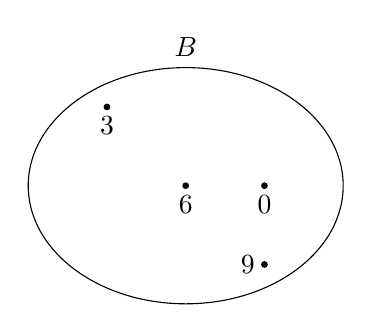
\begin{tikzpicture}[scale=1]
				\def\firstven{(0,0) ellipse (2cm and 1.5cm) }
				\draw \firstven ;
				\draw[fill=black](0,0)node[below]{$6$}circle(1pt)
				(1,0)node[below]{$0$}circle(1pt)
				(-1,1)node[below]{$3$}circle(1pt)
				(1,-1)node[left]{$9$}circle(1pt)
				(0,2)node[below]{$B$}
				;
		\end{tikzpicture}}
	}
\end{ex}
%%%=============================%%%

%%%=============EX_8=============%%%
\begin{ex}%[0D1H2-3]%[Dự án dề cương 3 Khối NH24-25-Đợt 2-Võ Thị Thùy Trang]
	Dùng các kí hiệu đoạn, khoảng, nửa khoảng, viết các tập hợp sau đây:
	\begin{listEX}[2]
		\item $\left\lbrace x \in \mathbb{R}\ \mid |\-2 \pi<x \leq 2 \pi\right\rbrace $;
		\item $\left\lbrace x \in \mathbb{R}\ \mid |x| \leq \sqrt{3}\right\rbrace$;
		\item $\left\lbrace x \in \mathbb{R}\ \mid |\ x<0\right\rbrace $;
		\item $\left\lbrace x \in \mathbb{R}\ \mid |\ 1-3 x \leq 0\right\rbrace $.
	\end{listEX}
	\loigiai{
		\begin{enumerate}
			\item Ta có $\{x \in \mathbb{R} \mid-2 \pi<x \leq 2 \pi\}=\left(-2\pi;2 \pi\right]$.
			\item Ta có $\left\lbrace x \in \mathbb{R}\ \mid |x| \leq \sqrt{3}\right\rbrace =\left[-\sqrt{3};\sqrt{3}\right]$.
			\item Ta có $\left\lbrace x \in \mathbb{R}\ \middle|\ x<0\right\rbrace =(-\infty;0)$.
			\item Vì $1-3x\leq 0\Leftrightarrow x\geq \dfrac{1}{3}$ nên $\left\lbrace x \in \mathbb{R}\ \mid |\ 1-3 x \leq 0\right\rbrace =\left[\dfrac{1}{3};+\infty\right)$.
		\end{enumerate}
	}
\end{ex}
%%%=============================%%%

%%%=============EX_9=============%%%
\begin{ex}%[0D1H2-3]%[Dự án dề cương 3 Khối NH24-25-Đợt 2-Võ Thị Thùy Trang]
	Hãy đọc tên, kí hiệu và biểu diễn mỗi tập hợp sau trên trục số:
	\begin{enumerate}
		\item $A=\{x \in \mathbb{R} \mid-2<x \leq 3\}$;
		\item $B=\{x \in \mathbb{R} \mid-3 \leq x \leq 1\}$;
		\item $C=\{x \in \mathbb{R} \mid 2 x-1>0\}$.
	\end{enumerate}
	\loigiai{
		\begin{enumerate}
			\item Tập hợp $A$ là nửa khoảng $(-2 ; 3]$ và được biểu diễn là
			\begin{center}
				\tikz{\draw[-stealth] (0,0)--(6,0);
					\path (2,0)node{$\Big($} +(90:0.5) node{$-2$}--(4,0) node{$\Big]$} +(90:.5) node{$3$};
					\path (3,0)node{} +(90:0.5) node{$0$};
					\fill[pattern=north east lines] (0,-4pt) rectangle (1.97,4pt) (4,-4pt) rectangle (6,4pt); }\\
			\end{center}
			\item Tập hợp $B$ là đoạn $[-3; 1]$ và được biểu diễn là
			\begin{center}
				\tikz{\draw[-stealth] (0,0)--(6,0); \path (2,0)node{$\Big[$} +(90:0.5) node{$-3$}--(4,0) node{$\Big]$} +(90:.5) node{$1$};
					\path (3,0)node{} +(90:0.5) node{$0$};
					\fill[pattern=north east lines] (0,-4pt) rectangle (2,4pt) (4,-4pt) rectangle (6,4pt); }
			\end{center}
			\item Tập hợp $C$ là khoảng $\left(\dfrac{1}{2} ;+\infty\right)$ và được biểu diễn là
			\begin{center}
				\tikz{\draw[-stealth] (0,0)--(6,0); \path (2,0)node{$\Big($} +(90:0.5) node{$\frac12$};
					\fill[pattern=north east lines] (0,-4pt) rectangle (1.97,4pt); }\\
			\end{center}
		\end{enumerate}
	}
\end{ex}
%%%=============================%%%

%%%=============EX_10=============%%%
\begin{ex}%[0D1V2-2]%[Dự án D - Đề cương 3 khối 10-11-12 NH25-26 đợt 1-Nguyễn Thanh Phong]
	Cho tập $A=(0 ;+\infty)$ và $B=\left\{x \in \mathbb{R} \mid m x^2-4 x+m-3=0\right\}$, $m$ là tham số. Tìm $m$ để $B$ có đúng hai tập con và $B \subset A$.
	\loigiai{Để $B$ có đúng hai tập con nghĩa là $B$ chỉ có duy nhất $1$ phần tử. Vì $\mathscr{P}(B)=2^1=2$. Lúc này bài toán quay về tìm $m$ để $B$ có duy nhất $1$ nghiệm thực dương. Khi đó, với:
		\begin{itemize}
			\item $m=0$ thì phương trình trở thành $-4x-3=0 \Rightarrow x=\dfrac{-3}{4} < 0$ (loại).
			\item $m \neq 0$ thì xét phương trình $mx^2-4x+m-3=0$. Để phương trình có duy nhất $1$ nghiệm thì $\Delta' = 0$. Khi đó:
			$$\Delta' =0 \Leftrightarrow 4-m(m-3)=0 \Leftrightarrow -m^2 + 3m + 4 =0 \Leftrightarrow \hoac{&m=-1 \\ &m=4.}$$
		\end{itemize}
		Kiểm tra:
		\begin{itemize}
			\item Với $m=-1$: $-x^2-4x-4=0 \Rightarrow x^2+4x+4=0 \Rightarrow (x+2)^2=0 \Rightarrow x=-2 < 0$ (loại).
			\item Với $m=4$: $4x^2-4x+1=0 \Rightarrow (2x-1)^2=0 \Rightarrow x=\dfrac{1}{2} > 0$ (thỏa mãn).
		\end{itemize}
		Vậy $m=4$.
	}
\end{ex}
%%%=============================%%%